%!TEX root = ../ArticleCalib_main.tex


%%%%%%%%%%%%% FIGURE 14  DOUBLEMENT STOCH


%%%%%%%%%%%%% TAU 1s

\begin{figure}[htbp]
\begin{center}
\captionsetup[subfigure]{position=top, labelfont=bf, textfont=normalfont, singlelinecheck=off, justification=raggedright }

\subfloat[]{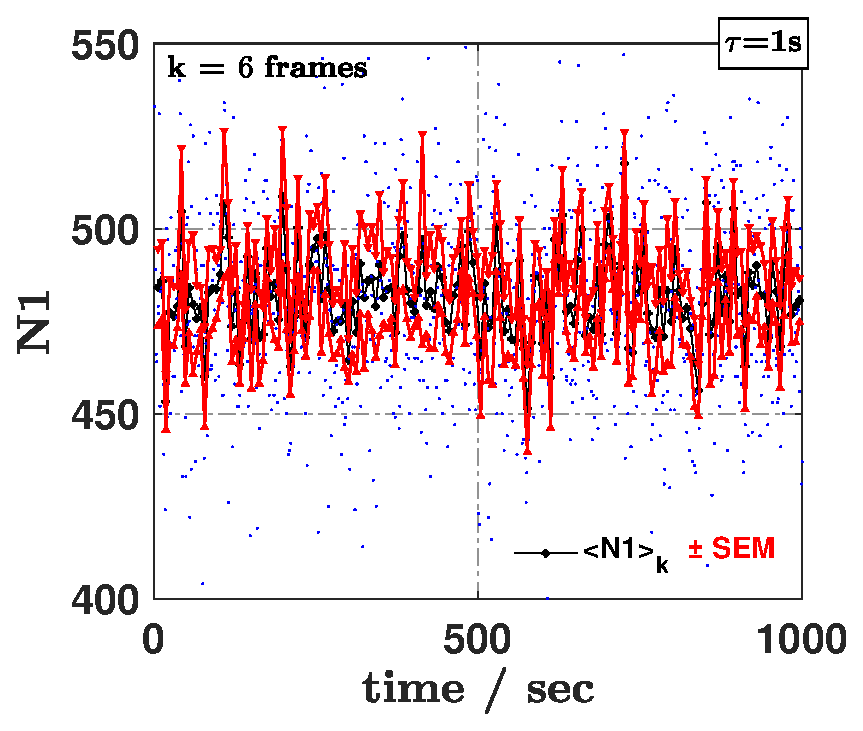
\includegraphics[width=0.4\linewidth]
	{fig14_doublementStoch/anlz191226_MeanSEM_BP_onk_doubleStoch_Tau1snoCRwithoutOutliers_1.eps}
	\label{fig:DoubleStoch:1s:A}} \qquad
\subfloat[]{\includegraphics[width=0.4\linewidth]
	{fig14_doublementStoch/anlz191226_MeanSEM_BP_onk_doubleStoch_Tau1snoCRwithoutOutliers_2.eps}
	\label{fig:DoubleStoch:1s:B}} \\

\subfloat[]{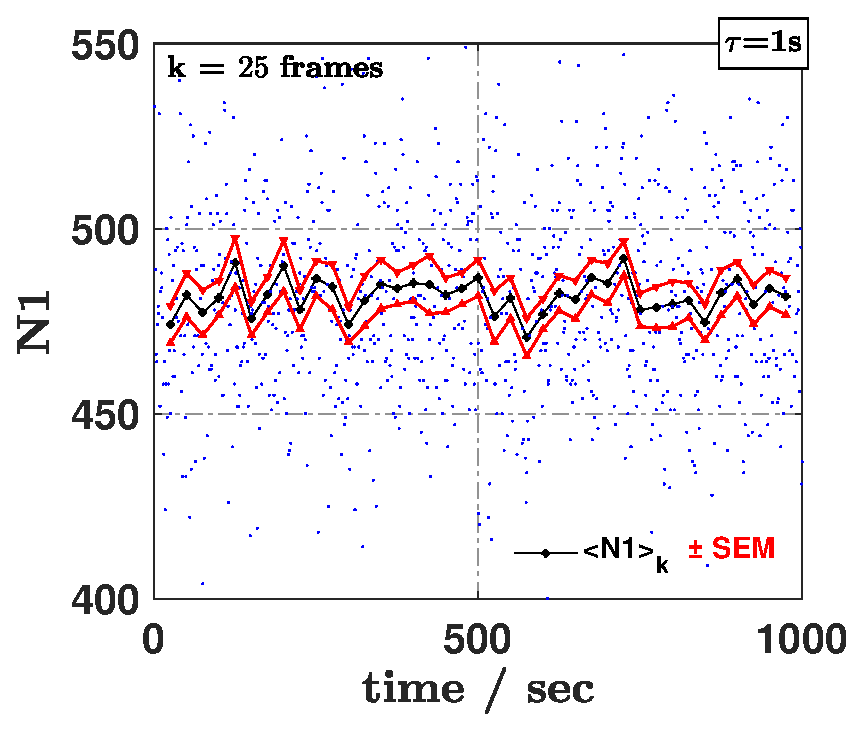
\includegraphics[width=0.4\linewidth]
	{fig14_doublementStoch/anlz191226_MeanSEM_BP_onk_doubleStoch_Tau1snoCRwithoutOutliers_3.eps}
	\label{fig:DoubleStoch:1s:C}} \qquad
\subfloat[]{\includegraphics[width=0.4\linewidth]
	{fig14_doublementStoch/anlz191226_MeanSEM_BP_onk_doubleStoch_Tau1snoCRwithoutOutliers_4.eps}
	\label{fig:DoubleStoch:1s:D}} \\

\subfloat[]{\includegraphics[width=0.4\linewidth]
	{fig14_doublementStoch/anlz191226_MeanSEM_BP_onk_doubleStoch_Tau1snoCRwithoutOutliers_5.eps}
	\label{fig:DoubleStoch:1s:E}} \qquad
\subfloat[]{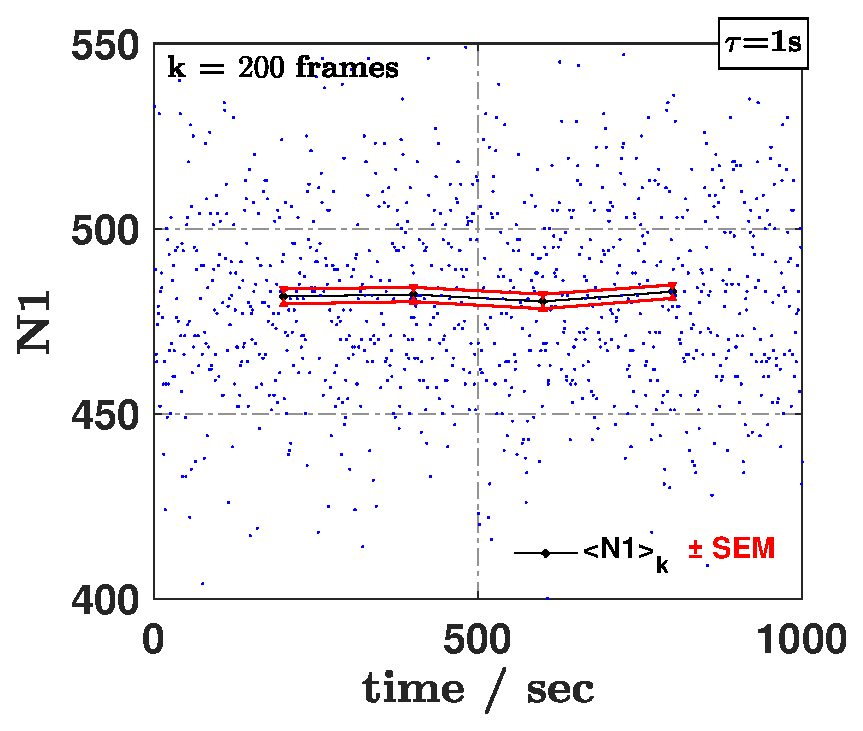
\includegraphics[width=0.4\linewidth]
	{fig14_doublementStoch/anlz191226_MeanSEM_BP_onk_doubleStoch_Tau1snoCRwithoutOutliers_6.eps}
	\label{fig:DoubleStoch:1s:F}} \\






\caption{
{\bf Stochastic Filter ($\tau = $ 1s) }.  
During background camera measurement, moving average of the total counts on the sensor ($<N1>_k$) for  k data points (N1, blue dots) and its standard deviation of the mean (SEM) during $\tau=$1second. 
Increasing k shows that significative fluctuations are detectable during time while increasing the period until 200 seconds for a $\tau = $ 1s \subref{fig:DoubleStoch:1s:F}.
}
\label{fig:DoubleStoch:1s}
\end{center}
\end{figure}





%%%%%%%%%%%%%%%%%%%%%%%%% TAU 100sec
\begin{figure}[htbp]
\begin{center}
\captionsetup[subfigure]{position=top, labelfont=bf, textfont=normalfont, singlelinecheck=off, justification=raggedright }


\subfloat[]{\includegraphics[width=0.4\linewidth]
	{fig14_doublementStoch/anlz191226_MeanSEM_BP_onk_doubleStoch_Tau100snoCRwithoutOutliers_1.eps}
	\label{fig:DoubleStoch:100s:A}} \qquad
\subfloat[]{\includegraphics[width=0.4\linewidth]
	{fig14_doublementStoch/anlz191226_MeanSEM_BP_onk_doubleStoch_Tau100snoCRwithoutOutliers_2.eps}
	\label{fig:DoubleStoch:100s:B}} \\

\subfloat[]{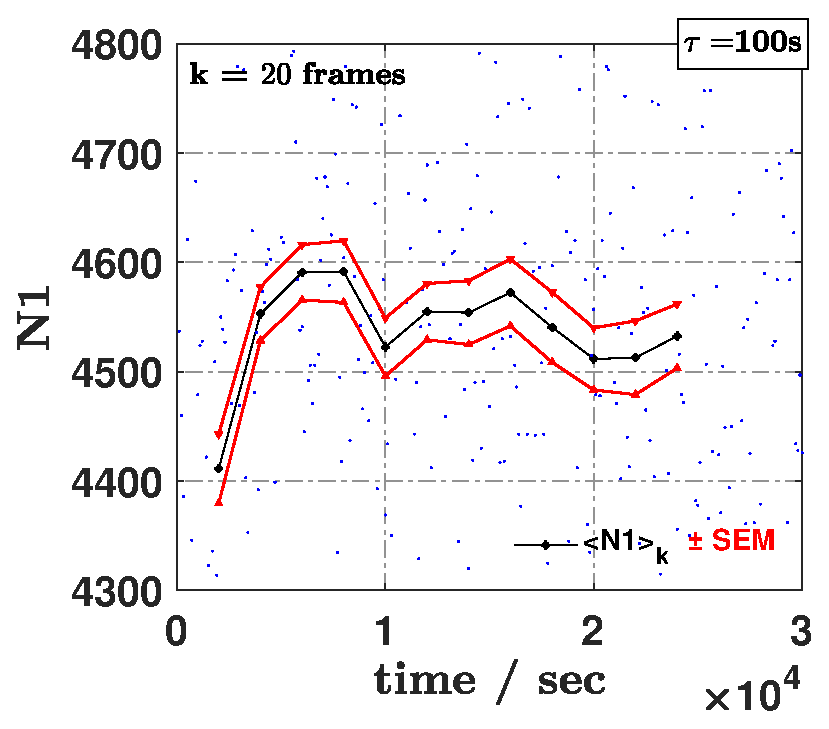
\includegraphics[width=0.4\linewidth]
	{fig14_doublementStoch/anlz191226_MeanSEM_BP_onk_doubleStoch_Tau100snoCRwithoutOutliers_3.eps}
	\label{fig:DoubleStoch:100s:C}} \qquad
\subfloat[]{\includegraphics[width=0.4\linewidth]
	{fig14_doublementStoch/anlz191226_MeanSEM_BP_onk_doubleStoch_Tau100snoCRwithoutOutliers_4.eps}
	\label{fig:DoubleStoch:100s:D}} \\

\subfloat[]{\includegraphics[width=0.4\linewidth]
	{fig14_doublementStoch/anlz191226_MeanSEM_BP_onk_doubleStoch_Tau100snoCRwithoutOutliers_5.eps}
	\label{fig:DoubleStoch:100s:E}} \qquad
\subfloat[]{\includegraphics[width=0.4\linewidth]
	{fig14_doublementStoch/anlz191226_MeanSEM_BP_onk_doubleStoch_Tau100snoCRwithoutOutliers_6.eps}
	\label{fig:DoubleStoch:100s:F}} \\


\caption{
{\bf Stochastic Filter ($\tau = $ 100s) }.  
During background camera measurement, moving average of the total counts on the sensor ($<N1>_k$) for  k data points (N1, blue dots) and its standard deviation of the mean (SEM) during $\tau=$100second. 
Increasing k shows that significative fluctuations are detectable during time while increasing the period until 8000  seconds for a $\tau = $ 100s \subref{fig:DoubleStoch:100s:F}.
}
\label{fig:DoubleStoch:100s}
\end{center}
\end{figure}





